\chapter{Stokes Structures}
A great overview of this topic is given in
\cite{Varadarajan96linearmeromorphic}.

Stokes structures are the \rewrite{necessary information} for meromorphic
classification.

%%%%%%%%%%%%%%%%%%%%%%%%%%%%%%%%%%%%%%%%%%%%%%%%%%%%%%%%%%%%%%%%%%%%%%%%%%%%%%%
\section{Situation}
Let $\cM^{nf}$ be a fixed model with the corresponding connection matrix
$A^0$.
We have the following commutative diagram of isomorphisms.
\begin{center}
  \begin{tikzpicture}[scale=3]
    \node[] (modSpcMat) at (0,0) {$\cH(A^0)$};
    \node[purple] (class) at (1,0) {$G\backslash\hat G(A^0)$};
    \node[green!40!black] (sheaf) at (3,1) {$\St(\cM^{nf})$};
    \node[] (sheaf2) at (2,1) {$H^1(S^1;\Lambda^{<0}(A^0))$};
    \node[blue] (mat) at (3,-1) {$\prod_{\theta\in\A}\Sto_\theta(A^0)$};
    \node[blue] (mat') at (3.5,-1.5) {$(U_+\times U_-)^{k-1}$};

    % \draw[thick,double] (modSpcMat) -- (modSpcSheaf) -- (class) -- (class2) --
    %   (modSpcMat);
    \draw[thick,double,blue] (modSpcMat) -- (class);
    \draw[thick,double] (sheaf) -- (sheaf2) node[midway,above] {\tiny def.};

    \draw[->,green!40!black] (modSpcMat) -- (sheaf);
    \draw[->,blue,dashed] (modSpcMat) edge[bend right=20] (mat);
    \draw[->,blue] (class) -- (mat);
    \draw[->,blue,dotted] (mat) -- (mat') node[midway,right] {$\cK=\{k-1\}$};
    \draw[->,purple,dashed] (class) -- (sheaf);
    % \draw[->,purple,dashed] (class) -- (mat);
    \draw[->,purple] (mat) -- (sheaf);
    \draw[->,purple,dashed] (sheaf) edge[bend right=20] (mat);

    \node[green!40!black] at (1,0.7) {\cite{sabbah2007isomonodromic}};
    \node[blue] at (2.3,-1.3) {\cite{thboalch},\cite{boalch}};
    \node[purple] at (3.5,0) {\cite{Loday1994}{\footnotesize(\cite{Loday2014})}};
  \end{tikzpicture}
\end{center}

\begin{comment}
  Matrizen Sicht:
  \begin{itemize}
    \item \cite{thboalch} and \cite[Chapter 3]{boalch}
      \\ largely following:
      \begin{itemize}
        \item[\textbf{8}] D.G. Babbitt and V.S. Varadarajan.
        \textbf{Formal reduction theory of meromorphic differential equations:
          a group theoretic view.}
        \texttt{euclid.pjm.1102720203.pdf}
        \item[\textbf{11}] \cite{BJL1979Birkhoff}
        \item[\textbf{40}] M. Jimbo, T. Miwa, and Kimio Ueno.
        \textbf{Monodromy preserving deformations of linear differential
          equations with rational coefficients I.}
        \item[\textbf{43}] \cite{Loday1994}
        \item[\textbf{50}] J. Martinet and J.P. Ramis.
        \textbf{Elementary acceleration and multisummability.}
      \end{itemize}
    \item \cite{van2003galois}
    \item Marius van der Put, Kyoshi Saito => Diff.Galois Theory
  \end{itemize}
  Moderne Sicht (sheaf-view):
  \begin{multicols}{2}
    \begin{itemize}
      \item Malgrange
      \item \cite{sabbah_cimpa90}, \cite{sabbah2007isomonodromic} and
        \cite{sabbah2009introduction,sabbah2013introduction}
    \end{itemize}
  \end{multicols}
  and
  \begin{multicols}{2}
    \begin{itemize}
      \item \cite{LodayRichaud2004,Loday2014}
      \item \cite{Remy2014} (\textbf{3 explicit} examples! \TODO{})
    \end{itemize}
  \end{multicols}
  See also:
  \begin{multicols}{3}
    \begin{itemize}
      \item \cite{Loday1994} for \textbf{Sheaf $\to$ Matrix}
      \item \cite{Varadarajan96linearmeromorphic} for \textbf{overview of both}
      \item looks at $\infty$: \cite{sibuya1990Linear,BJL1979Birkhoff}
    \end{itemize}
  \end{multicols}
\end{comment}

%%%%%%%%%%%%%%%%%%%%%%%%%%%%%%%%%%%%%%%%%%%%%%%%%%%%%%%%%%%%%%%%%%%%%%%%%%%%%%%
\section{Stokes structures: Malgrange-Sibuya isomorphism}
\begin{comment}
  \cite[Thm.I.2.1]{Loday1994}, \cite[Thm.4.3.9]{Loday2014} and
  \cite[Thm.II.6.2]{sabbah2007isomonodromic}
\end{comment}
Here we will look at the classifying set and we will proof, that it is
isomorphic \TODO[as\dots] to the first non abelian cohomology \rewrite{set}
$H^1(S^1;\Lambda^{<0}(A^0))=:\St(A^0)$.

Let us first define a Stokes sheaf $\Lambda(A^0)$ on $S^1$, as the sheaf of
flat isotropies.
\begin{defn} \label{defn:StokesSheaf}
  The Stokes sheaf $\Lambda(A^0)$ of $A^0$, is the sheaf of groups defined on
  $S^1$ whose stalk at any point $\theta\in S^1$ is the group of germs of
  $f\in\Gl_n(\cO(\mathfrak{s}))$, $\mathfrak{s}$ a sector containing $\theta$, satisfying
  the conditions:
  \begin{enumerate}
    \item Flatness: $\underset{x\in\mathfrak{s}}{\underset{x\to0}{\lim}}f(x)=1$
      and $f\sim_{\mathfrak{s}} 1$;
    \item Isotropy of $A^0$: ${}^f\!A^0=A^0$.
  \end{enumerate}
  \begin{comment}
    \begin{s-rem}
      $\Lambda(A^0)$ is the same as $\Aut^{<0}(\tilde\cM^{nf})$
      in~\cite{sabbah2007isomonodromic} which is defined as follows \TODO
    \end{s-rem}
  \end{comment}
\end{defn}

\subsection{The theorem}
\begin{comment}
  \TODO[See \cite{thboalch} for sheaf-less definition]
\end{comment}
Let $(\cM,\nabla,\hat f)$ be a marked germ of a  meromorphic connection.
There exists an open covering $\cU=(U_j)_{j\in J}$ and for every open set an
isomorphism
\[
  f_j:(\tilde\cM,\tilde\nabla)_{|U_j}
  \to(\tilde\cM^{nf},\tilde\nabla^{nf})_{|U_j}
\]
such that $\hat f_j=f$. By $(f_kf_j^{-1})_{jk}$ is then a cocycle of the
sheaf $\St(A^0)$, relative to the covering $\cU$, defined.
For other lifts $f_j'$ of $\hat f$ on $W_j$, $(f_j'f_j^{-1})$ is a $0$-cochain
of $\Sto(A^0)$ relative to $\cU$. Thus the associated cochians to $(f_j)$ and
$(f_j')$ are equivalent. One can also check that, if $(\cM,\nabla,\hat f)$ and
$(\cM',\nabla',\hat f')$ are isomorphic, the corresponding cocycles define the
same cohomology class. This defines a mapping of pointed sets
to the first non abelian cohomology of $\Lambda^{<0}(A^0)$
\[
  \cH\to H^1(S^1;\Lambda^{<0}(A^0)) \,,
\]
which sends the class of $(\cM^{nf},\nabla^{nf},\hat\id)$ to that of
$\id$.

\begin{tthm}[Malgrange-Sibuya] \label{thm:mainThm1}
  The homomorphism
  \[
    \exp:\cH\to\St(A^0):=H^1(S^1;\Lambda^{<0}(A^0))
  \]
  is an isomorphism of pointed\footnote{Which maps the class of
  $(\cM^{nf},\nabla^{nf},\hat\id)$ to that of $\id$, i.e.\ the trivial
  cohomology class.} sets.
\end{tthm}
\begin{comment}
  \begin{rem}
    \marginnote{\cite{Loday1994} Remark I.2.2}
    To another normal form $A^1={}^\Phi\!A^0$ there correspond cochains which
    are conjugated via $\Phi$.
    We get the following commutative diagram:
    \[ \begin{tikzcd}
        G\backslash\hat G(A^1) \rar{\cdot\Phi}\dar{\exp}
        & G\backslash\hat G(A^0) \dar{\exp}
        & \hat F \arrow[|->]{r}\arrow[|->]{d}
        & \hat F\Phi \arrow[|->]{d}
      \\ H^1(S^1;\lambda(A^1)) \rar
        & H^1(S^1;\lambda(A^0))
        & \exp_{\mu_1}(\hat F) \arrow[|->]{r}
        & \exp_{\mu_0}(\hat F\Phi)
    \end{tikzcd} \]
    where $\exp_{\mu_0}(\hat F\Phi)=\Phi^{-1}\exp_{\mu_0}(\hat F)\Phi$.
  \end{rem}
\end{comment}

\subsubsection{The theorem (system version)}
Since the language of meromorphic connections is equivalent to the one of
systems, there is also the translated version of the Malgrange-Sibuya
isomorphism to the language of systems.
\begin{comment}
  \begin{itemize}
    \item \TODO[See \cite{thboalch} for sheaf-less definition]
  \end{itemize}
\end{comment}
Let $(A,\hat F)$ be a marked pair, i.e. $\hat F$ solves $[A^0,A]$.
There exists an open covering $\cU=(U_j)_{j\in J}$ and for every open set
a lift $F_j\in\Gl_n(\cA(U_j))$ which solves $[A,A^0]$.
By $(F_kF_j^{-1})_{jk}$ is then a cocycle of the sheaf $\St(A^0)$, relative to
the covering $\cU$, defined.
For other lifts $F_j'$ of $\hat F$ on $U_j$, $(F_j'F_j^{-1})$ is a $0$-cochain
of $\Sto(A^0)$ relative to $\cU$.
Thus the associated cochians to $(f_j)$ and $(f_j')$ are equivalent.
One can also check that, if $(A,\hat F)$ and $(A',\hat F')$ are equivalent, the
corresponding cocycles define the same cohomology class.
This defines a mapping of pointed sets to the first non abelian cohomology of
$\Lambda^{<0}(A^0)$
\[
  \cH\to H^1(S^1;\Lambda^{<0}(A^0)) \,,
\]
which we call $\exp$.

\begin{tthm}[Malgrange-Sibuya] \label{thm:mainThm1}
  The homomorphism
  \[
    \exp:\cH\to\St(A^0):=H^1(S^1;\Lambda^{<0}(A^0))
  \]
  is an isomorphism of pointed\footnote{Which maps the class of
  $(A^0,\hat\id)$ to that of $\id$, i.e.\ the trivial cohomology class.} sets.
\end{tthm}
\begin{rem}
  \marginnote{\cite{Loday1994} Remark I.2.2}
  To another normal form $A^1={}^\Phi\!A^0$ there correspond cochains which
  are conjugated via $\Phi$.
  We get the following commutative diagram:
  \[ \begin{tikzcd}
      G\backslash\hat G(A^1) \rar{\cdot\Phi}\dar{\exp}
      & G\backslash\hat G(A^0) \dar{\exp}
      & \hat F \arrow[|->]{r}\arrow[|->]{d}
      & \hat F\Phi \arrow[|->]{d}
    \\ H^1(S^1;\lambda(A^1)) \rar
      & H^1(S^1;\lambda(A^0))
      & \exp_{\mu_1}(\hat F) \arrow[|->]{r}
      & \exp_{\mu_0}(\hat F\Phi)
  \end{tikzcd} \]
  where $\exp_{\mu_0}(\hat F\Phi)=\Phi^{-1}\exp_{\mu_0}(\hat F)\Phi$.
\end{rem}

\subsection{Proof}
We will mainly refer to \cite[section 6.d]{sabbah2007isomonodromic}, where a
slightly more complicated case, with deformation space, is proofen. Our proof is
obtained by choosing $X=\{0\}$ as the trivial deformation space.
\begin{comment}
  See also \cite{BJL1979Birkhoff} and \cite{babbitt1989local} although the proof
  goes back to work from Malgrange and Sibuya (see for example
  \cite{sibuya1990Linear}).
\end{comment}
\TODO[Define $\tilde\cM$ or find other way!]
\begin{proof}
  \textbf{First look at injectivity:}
  Consider the two elements $(\cM,\nabla,\hat f)$ and $(\cM',\nabla',\hat f')$
  of $\cH$ which map to same element
  \[
    \exp((\cM,\nabla,\hat f))=\lambda=\exp((\cM',\nabla',\hat f'))
      \in H^1(S^1;\Lambda^{<0}(A^0)) \,.
  \]
  Since \TODO{}, it is then possible to find a finite covering
  $\cU=\{U_j;j\in J\}$ of $S^1$ such that $\lambda$ is the class of the
  cocycles $(f_lf_j^{-1})$ and $(f_l',f_j'^{-1})$, where $f_j$,$f_j'$ are
  defined on $U_j$.
  Then there exists \TODO{} a $0$-cochain $(g_j)$ of the sheaf
  $\Aut^{<0}(\tilde\cM^{nf})$ relative to the covering $(I_j)$, such that
  \[
    f_l'f_j'^{-1}=g_lf_lf_j^{-1}g_j^{-1} \text{ on } I_j\cap I_l.
  \]
  If we set $\sigma=f_j^{-1}g_{j}^{-1}f_j'$ on $I_{j}$, we get a horizontal
  section, on \TODO{}
  Thus we have $\sigma\circ\hat{f'}=\hat f$ Therefore $(\cM,\nabla,\hat f)$ and
  $(\cM',\nabla',\hat{f'})$ are isomorphic and injectivity is proven.

  \textbf{Now look at surjectivity:}
  Exactly as in \cite{sabbah2007isomonodromic}\marginnote{Which refers to
  \cite{Malgrange1983}} we will start this part of the proof by giving a
  necessary and sufficient condition for a class $\lambda$ in
  $H^1(S^1,\Lambda^{<0}(A^0))$
  \TODO[$\Lambda^{<0}(A^0)\hat{=}\Aut^{<0}(\tilde\cM^{nf})$ or
  $\Aut^{<0}(\cM^{nf})$?]
  to come from an object
  $(\cM,\nabla,\hat f)\in\cH$:
  \begin{einr}
    This is the case if and only if the image of
    $\lambda\in\Aut^{<0}(\cM^{nf})$ in the set
    $H^1(S^1,\Aut_{\cA}(\tilde\cM^{nf}))$ (which contains only the
    $\cA$-linear automorphisms) is the identity.
  \end{einr}
  \begin{proof}
    \textbf{``\Rightarrow{}'':}
    If $\lambda$ is the image of some $(\cM,\nabla,\hat f)$ then there exists
    \begin{itemize}
      \item a covering $(I_{j})$ of $S^1$ and
      \item isomorphisms $f_j:\tilde\cM\overset{\sim}\to\tilde\cM^{nf}$
        inducing $\hat f$
    \end{itemize}
    such that $\lambda$ comes from a cocycle $(\lambda_{j,l})=(f_lf_j^{-1})$ on
    $I_j\cap I_l$.
    \TODO{} shows, that $(\lambda_{jl})$ is a coboundary of
    $\Aut_\cA(\tilde\cM^{nf})$.

    \textbf{``\Leftarrow{}'':}
    If for some suitable covering $(I_j)$ the cocycle $(\lambda_{jl})$ is a
    coboundary with values in $\Aut_\cA(\tilde\cM^{nf})$, i.e.\
    $\lambda_{jl}=f_lf_j^{-1}$, we define a new connection $\nabla$ on
    $\tilde\cM^{nf}$ by conjugating $\nabla^{nf}$ by $f_j$ on $I_j$.

    \TODO{}

    Moreover $\hat f_j=\hat f_l$ on $I_j\cap I_l$, so that the formal
    isomorphisms
    \[
      \hat f_j:(\hat \cM^{nf},\nabla)
      \overset{\sim}{\longrightarrow}
      (\hat\cM^{nf},\nabla^{nf})
    \]
    can be glued in an isomorphism $\hat f:(\hat \cM^{nf},\nabla)
    \overset{\sim}{\longrightarrow}(\hat\cM^{nf},\nabla^{nf})$.
  \end{proof}

  Thus, the proof of~\ref{thm:mainThm1} is a consequence of the following
  Malgrange-Sibuya theorem.
  \begin{thm}[Malgrange-Sibuya]
    \marginnote{\cite[Thm.II.6.10]{sabbah2007isomonodromic}}
    The image of the mapping
    \[
      H^1(S^1,\Gl_d^{<0}(\cA_{\tilde D}))
      \to
      H^1(H^1,\Gl_d(\cA_{\tilde D}))
    \]
    is the identity.
  \end{thm}
  \begin{proof}
     For which we refer to
     \cite[Th.A.1]{Malgrange1983},
     \cite[Th.6.4.1]{sibuya1990Linear},
     \cite{babbitt1989local}
  \end{proof}
\end{proof}

%%%%%%%%%%%%%%%%%%%%%%%%%%%%%%%%%%%%%%%%%%%%%%%%%%%%%%%%%%%%%%%%%%%%%%%%%%%%%%%
\section{The Stokes group}
%%%%%%%%%%%%%%%%%%%%%%%%%%%%%%%%%%%%%%%%%%%%%%%%%%%%%%%%%%%%%%%%%%%%%%%%%%%%%%%
\subsection{Anti-Stokes directions and the Stokes group}
\begin{comment}
  \cite[I.4]{Loday1994}
\end{comment}
We denote
\[
  \cQ_{[A^0]}
  :=
  \left\{q_1(t^{-1}),\dots,q_s(t^{-1})\right\}
  \,,
\]
where the $q_i$ are the diagonal elements of $Q$\footnote{$Q=\diag(
\underset{n_1\text{-times}}{\underbrace{q_1,\dots,q_1}},q_2,\dots ,q_s)$}
from \TODO{},
the set of the determining polynomials of $[A^0]$ and
\[
  \cQ_{[\End A^0]}:=\left\{\left(q_i-q_l\right)(t^{-1})
    \mid q_i \neq q_l \in\cQ_{[A^0]}
  \right\}
\]
the set of the determining polynomials of $[\End A^0]$ where\dots
\begin{defn}
  We call
  \begin{itemize}
    \item $a_{jl}\in\C\backslash\{0\}$ the \emph{leading factor},
    \item $\frac{a_{jl}}{t^{k}}=:q_{jl}(t^{-1})$ the \emph{leading
      coefficient} and
    \item $k=k_{jl}$ the \emph{degree} $\deg(q_j-q_l)$ of $(q_j-q_l)$ or a
      \emph{level} of $A^0$
  \end{itemize}
  of $q_j-q_l\in\cQ_{[\End A^0]}$ if
  \[
    q_j-q_l\in\left\{\frac{a_{jl}}{t^{k}}+h \mid h \in o(t^{-k})\right\}\,.
  \]
  \begin{s-rem}
    \begin{enumerate}
      \item It is obvious, that $k_{jl}=k_{lj}$ and
        $q_{jl}(t^{-1})=-q_{lj}(t^{-1})$.
      \item In \cite{boalch} and \cite{thboalch} the $k$ is always an integer
        and is incremented by one. We will prefer the other definition, which
        is taken from \cite{Loday1994}, because \TODO
      \item In \cite[Def.4.3.6]{Loday2014} $a_{jl}$ gets a negative sign to
        be consistend with calculations at $\infty$. Here this is not
        necessary, since we use the clockwise ordering of points on $S^1$
        (cf.~\ref{defn:antiStokesDir}).
        \begin{comment}
          Does that mean, that, to be consistend with \cite{boalch}, one has to
          invert the permutation matrix?
        \end{comment}
    \end{enumerate}
  \end{s-rem}
  The degrees of the elements in $\cQ_{[\End A^0]}$ are the
  \emph{levels} of $A^0$.
  The set of all levels of $A^0$ will be denoted by
  \[
    \cK=\{k_1<\dots<k_r\} \subset \Q \,.
  \]
  \begin{s-rem}
    $A^0$ is unramified if and only if $\cK\subset\Z$. Since we only look at
    the unramified case, this will be always the case.
  \end{s-rem}
\end{defn}

\begin{defn}
  \begin{comment}
    See \cite{hotta2008}
  \end{comment}
  A function is \emph{of maximal decay}, if \TODO{}

  A function is \emph{flat}, if \TODO{}
\end{defn}

On the elements of $\cQ(A^0)$ we define the following (partial) order
relations:
\begin{defn}
  \marginnote{\cite[Def.I.4.4]{Loday1994}}
  Let $\tilde\theta$ be a determination of $\theta$.
  We define the relations
  \begin{itemize}
    \item $\boldmath q_j \underset{\tilde\theta}{\prec} q_l$
      :\Leftrightarrow{} $\Re(a_{jl}e^{-ik_{jl}\tilde\theta})<0$
    \\\Leftrightarrow{} $e^{(q_j-g_l)(t^{-1})}$ is
      flat at $0$ in a neighbourhood of the direction $\tilde\theta$.
    \item $\boldmath q_j \underset{\tilde\theta,\max}{\prec} q_l$
      :\Leftrightarrow{} $a_{jl}e^{-ik_{jl}\tilde\theta}$ is a real negative
      number, i.e.\ $q_j \underset{\tilde\theta}{\prec} q_l$ and
      $\Im(a_{jl}e^{-ik_{jl}\theta})=0$.
      \\\Leftrightarrow{} $e^{(q_j-g_l)(t^{-1})}$ is of maximal
      decay in the direction $\tilde\theta$.
      \begin{comment}
        \Leftrightarrow{} $q_{jl}(t^{-1})\in\R_{<0}$ along $\tilde\theta$.
      \end{comment}
      \begin{s-rem} \label{rem:rotationalSym}
        \marginnote{\cite[8]{thboalch}}
        Let $\theta\in S^1$ with determination $\tilde\theta$.
        Let $(j,l)$ be a pair such that
        $q_j \underset{\tilde\theta,\max}{\prec} q_l$, i.e.\ such that
        $a_{jl}e^{-ik_{jl}\tilde\theta}\in\R_{<0}$.
        Hence, for $n\in\N$,
        \begin{align*}
          a_{jl}e^{-ik_{jl}\left(\tilde\theta+n\frac{\pi}{k_{jl}}\right)}
          &=a_{jl}e^{-ik_{jl}\tilde\theta}e^{-in\pi}
          = \begin{cases}
            a_{jl}e^{-ik_{jl}\tilde\theta}\in\R_{<0} 
              & \text{, if $n$ is even}
          \\-a_{jl}e^{-ik_{jl}\tilde\theta}\in\R_{>0} 
              & \text{, if $n$ is uneven}
          \end{cases}
        \end{align*}
        is, in the case when $n$ is even, also real and negative. In the other
        case, when $n$ is uneven, we use that $a_{jl}=-a_{lj}$ and
        $k_{jl}=k_{lj}$ to obtain
        $a_{lj}e^{-ik_{jl}\left(\tilde\theta+n\frac{\pi}{k_{lj}}\right)}
        \in\R_{<0}$.

        Thus, for $\tilde\theta'=\tilde\theta+n\frac{\pi}{k_{jl}}$ as
        determination of $\theta'=\theta+n\frac{\pi}{k_{jl}}$, we have
        \begin{itemize}
          \item $q_j \underset{\tilde\theta',\max}{\prec} q_l$ when $n$ is even
            or
          \item $q_l \underset{\tilde\theta',\max}{\prec} q_j$ when $n$ is
            uneven.
        \end{itemize}
      \end{s-rem}
  \end{itemize}
  \begin{s-rem}
    In the unramified case these relations do not depend on the determination
    $\tilde\theta$ of $\theta$. As a consequence we will only write
    $\underset{\theta}{\prec}$ and $\underset{\theta,\max}{\prec}$.
  \end{s-rem}
\end{defn}

\begin{defn}
  \label{defn:antiStokesDir}
  % \marginnote{See \cite[Def.I.4.5]{Loday1994}(for the ramified case)
  %   \cite[Def.3.2]{boalch}}
  \begin{enumerate}
    \item $\theta$ is an \emph{anti-Stokes direction} if there is at least one
      pair $(q_j,q_l)$ in $\cQ(A^0)$, which satisfies
      $q_j \underset{\theta,\max}{\prec} q_l$.
      \begin{itemize}
        \item Let $\A=\{\theta_1,\dots,\theta_{\nu}\}$ denote the set of all
          anti-Stokes directions in a clockwise ordering. For a uniform
          notation later, \rewrite{define $\A$ to contain a single, arbitrary
          direction if $\cK=\{0\}$.}
          \TODO[make all Stokes dirs $\alpha$ instead of $\theta$?]
          \begin{s-rem} \label{rem:rotationalSymPrime}
            \begin{enumerate}
              \item From remark~\ref{rem:rotationalSym} follows, that in the
                case $\cK=\{k\}$, the set $\A$ has $\frac{\pi}{k}$-rotational
                symmetry.
              \item The clockwise ordering is chosen, similar to
                \cite{Loday1994}, since the calculations are then compatible
                with the calculations, which look at $\infty$ and take a
                counterclockwise ordering. \cite{boalch} and \cite{thboalch}
                use the inverse ordering, but look also at $0$.
                In \cite{Loday2014} this problem is solved by an additional
                minus sign\comm{~to $a_{ij}$}.
            \end{enumerate}
          \end{s-rem}
      \end{itemize}
    \item $\theta$ is an \emph{Stokes direction} when there is at least one
      pair $(q_j,q_l)$ in $\cQ(A^0)$, which satisfies neither
      $q_j\underset{\theta}{\prec} q_l$ nor $q_l\underset{\theta}{\prec} q_j$.
      \begin{itemize}
        \item Let $\S=\{\sigma_1<\cdots<\sigma_\mu\}$ be the set of Stokes
          directions.
      \end{itemize}
  \end{enumerate}
\end{defn}

\begin{comment}
  In the case with only one level, the stokes directions are rotational
  symetric.
  \\The stokes direction, beared by level $k$ have the rotational symmetry.
\end{comment}

As a \rewrite{subgroup of the stalk at $\theta$} of the in
definition~\ref{defn:StokesSheaf} defined Stokes sheaf $\Lambda^{<0}(A^0)$ we
define the Stoken group as follows.
\begin{defn}
  Define the \emph{Stokes group}
  \[
    \Sto_\theta(A^0):=
    \left\{\phi_\theta\in\Lambda_\theta^{<0}(A^0)
      \mid \phi_\theta \text{ has maximal decay at } \theta
    \right\} \,.
  \]
  \begin{s-rem}
    \begin{enumerate}
      \item For $\theta\notin\A$ the group $\Sto_\theta(A^0)$ is trivial, since
        no flat isotropy has maximal decay, but the identity.
      \item This is in fact a group, since \TODO{}
    \end{enumerate}
  \end{s-rem}
\end{defn}

%%%%%%%%%%%%%%%%%%%%%%%%%%%%%%%%%%%%%%%%%%%%%%%%%%%%%%%%%%%%%%%%%%%%%%%%%%%%%%%
\subsection{Faithful representation of the Stokes group}
\begin{comment}
  See \cite[9f]{thboalch} and \cite[??]{Loday1994}
\end{comment}
\begin{defn}
  Define the group
  \[
    \SSto_\theta(A^0)= \left\{K\in G\mid K_{jl}=\delta_{jl} \text{ unless }
      q_j \underset{\theta,\max}{\prec} q_l \right\}
  \]
  which will arise as a faithful representation (cf.\
  section~\ref{sec:faithRepre}) of $\Sto_\theta(A^0)$.
\end{defn}
Let $X_0=t^L e^{Q(t^{-1})}$ be \rewrite{the normal solution corresponding to
$A^0$} (cf.\ definition~\ref{defn:normSol}).
For every determination $\tilde\theta$ of $\theta$ we denote by
$X_{0,\tilde\theta}$ the function defined by $X_0$ with that determination of
the argument near the direction $\theta$.

\begin{prop} \label{prop:representation}
  \marginnote{\cite[Def.I.4.7]{Loday1994}\\\cite[78f]{Loday2014}}
  In this situation the morphism
  \begin{align*}
    \rho_{\tilde\theta}:\Sto_\theta(A^0)&\to\SSto_\theta(A^0)
    \\\phi_\theta
    &\mapsto 1+C_{\tilde\theta}
    :=e^{-Q(t^{-1})}t^{-L} \phi_\theta t^L e^{Q(t^{-1})}
  \end{align*}
  is an isomorphism which maps a germ of $\Sto_\theta(A^0)$ to the unique
  matrix $1+C_{\tilde\theta}$ such that
  \begin{equation} \label{eq:representation}
    \phi_\theta(t)X_{0,\tilde\theta}(t)
    =X_{0,\tilde\theta}(t)(1_n+C_{\tilde\theta})
  \end{equation}
  near $\theta$.  We call the matrux $1+C_{\tilde\theta}$ a
  \emph{representation of $\phi_\theta$}.
  \begin{s-rem}
    \begin{enumerate}
      \item \marginnote{\cite[10]{thboalch}}
        The morphism $\rho_{\tilde\theta}$ relates solutions $\phi_\theta$ of
        $[\End(A^0)]=[A^0,A^0]$ to solutions of $[0,0]$ which are the constant
        matrices $G$.
      \item This morphism depends on the choice of the determination
        $\tilde\theta$ of $\theta$.
    \end{enumerate}
  \end{s-rem}
\end{prop}
\begin{proof}
  In general, the map $\rho_{\tilde\theta}$ maps to the $G$ since
  \rewrite{conjugation} by the fundamental solution yields a constant matrix.
  To see that the obtained matrix has the necessary zeros, to lie in
  $\SSto_{\theta}(A^0)$ we look at equation (\ref{eq:representation}) and
  deduce
  \[
    \phi_\theta(t)
    =t^L e^{Q(t^{-1})}(1_n+C_{\tilde\theta})e^{-Q(t^{-1})}t^{-L}
  \]
  with the given choice of the argument near $\theta$.
  After decomposing $C_{\tilde\theta}$ into
  \begin{align*}
    C_{\tilde\theta}&=\begin{pmatrix}
      c_{(1,1)} & c_{(1,2)} & \cdots &\\
      c_{(2,1} & \ddots\\
      \vdots \\
      & & & c_{(s,s)}
    \end{pmatrix}
  \\&=
    \underset{C_{\tilde\theta}^{(1,1)}}{\underbrace{%
      \begin{pmatrix}
        c_{(1,1)} & 0 & \cdots &\\
        0\\
        \vdots&\\
        &
      \end{pmatrix}
    }}
    +
    \underset{C_{\tilde\theta}^{(1,2)}}{\underbrace{%
      \begin{pmatrix}
        0 & c_{(1,2)} & 0 & \cdots\\
        & 0 &\\
        &\vdots\\
        &
      \end{pmatrix}
    }}
    +\cdots+
    \underset{C_{\tilde\theta}^{(s,s)}}{\underbrace{%
      \begin{pmatrix}
        &\\
        & & & \vdots\\
        & & & 0\\
        & \cdots & 0 & c_{(s,s)}
      \end{pmatrix}
    }}
  \\&=\sum_{(l,j)}C_{\tilde\theta}^{(l,j)}
  \end{align*}
  where the $c_{(j,l)}$ are blocks of size $n_j\times n_l$ which correspond to
  the structure of $Q$, we get
  \[
    \phi_\theta=
      t^L\left(
        1_n+\sum_{(l,j)}C_{\tilde\theta}^{(l,j)}e^{(q_l-q_j)(t^{-1})}
      \right)t^{-L} \,.
  \]
  \begin{comment}
    \begin{align*}
      \phi_\theta(t)
      &=t^Le^{Q(t^{-1})}\left(
        1_n+C_{\tilde\theta}
      \right)e^{-Q(t^{-1})}t^{-L}
    \\&=t^Le^{Q(t^{-1})}\left(
        1_n+\sum_{(l,j)}C_{\tilde\theta}^{(l,j)}
      \right)e^{-Q(t^{-1})}t^{-L}
    \\&=t^L\left(
        1_n+\sum_{(l,j)}e^{Q(t^{-1})}C_{\tilde\theta}^{(l,j)}e^{-Q(t^{-1})}
      \right)t^{-L}
    \\&=t^L\left(
          1_n+\sum_{(l,j)}C_{\tilde\theta}^{(l,j)}e^{(q_l-q_j)(t^{-1})}
        \right)t^{-L} \,.
    \end{align*}
  \end{comment}
  Thus, for $\phi_{\theta}$ to be flat in direction $\theta$, it is
  necessary and sufficient that if $e^{(q_l-q_j)(t^{-1})}$ does not have
  maximal decay in direction $\tilde\theta$ the corresponding
  block $C_{\tilde\theta}^{(l,j)}$ vanishes.

  \TODO[Proof isom? faithfulness?]
  \rewrite{It is clearly a bijection, since the
  conjungation by the inverse of the fundamental solution is a inverse
  morphism.}
\end{proof}

In particular we get, that
\begin{itemize}
  \item for $j=l$ are the (diagonal) blocks $C_{\tilde\theta}^{(l,j)}$ vanish
    since $q_l-q_j=0$ does not have maximal decay and
  \item if $e^{q_j-q_l}$ has has maximal decay, then $e^{q_l-q_j}$ has not.
    Thus if $C_{\tilde\theta}^{(l,j)}$ is not equal to zero, the block
    $C_{\tilde\theta}^{(j,l)}$ is necessarily zero.
\end{itemize}
\begin{rem}
  This implies that the matrix $1_n+C_{\tilde\theta}$ is unipotent.
  \rewrite{Thus $\Sto_\alpha(A^0)$ is a unipotent Lie group.}
\end{rem}
On the other hand, every constant unipotent Matrix, with zeros at the necessary
positions, characterizes a unique element of $\Sto_\theta(A^0)$.

\begin{lem}
  \TODO[lemma or corollary?]
  \marginnote{\cite[Def.I.4.12]{Loday1994}}
  A germ $\phi_\theta\in\Lambda_\theta(A^0)$ is a Stokes germ, i.e.\ an element
  in $\Sto_\theta(A^0)$ if and only if for some, hence all determination
  $\tilde\theta$, it has a representation $1+C_{\tilde\theta}$ where
  \[
    C_{\tilde\theta}=\sum_{(l,j)\mid q_j\underset{\tilde\theta,\max}{\prec}q_l}
    C_{\tilde\theta}^{(l,j)}
  \]
  and $C_{\tilde\theta}^{(l,j)}$ have the necessary block structure.
\end{lem}

%%%%%%%%%%%%%%%%%%%%%%%%%%%%%%%%%%%%%%%%%%%%%%%%%%%%%%%%%%%%%%%%%%%%%%%%%%%%%%%
\subsection{Filtration of the Stokes group by levels}
\begin{comment}
  See
  \cite{Loday1994}
  and
  \cite[362ff]{Martinet1991}
\end{comment}
We denote the set of \emph{levels of the germ}
$\phi_{\theta}\in\Sto_\theta(A^0)$ by
\[
  \cK(\phi_\theta):= \left\{\deg(q_j-q_l)\mid C_{\tilde\theta}^{(l,j)}\neq0
    \text{ in some determination of }\phi_\theta\right\} \subset \cK
\]
\begin{defn}
  A germ $\phi_\theta$ is called a \emph{$k$-germ} when
  $\cK(\phi_{\theta})\subset\{k\}$, i.e.\ its only level, if existent, is $k$.
\end{defn}

\begin{notations}
  \marginnote{\cite[Not.I.4.15]{Loday1994},\\\cite[362]{Martinet1991}}
  For $k\in\cK$ and $\theta\in\A$ we set:
  \begin{itemize}
    \item $\Lambda^{k}(A^0):=$ the subsheaf of $\Lambda(A^0)$ of all germs,
      which are generated by $k$-germs;
    \item $\Lambda^{\leq k}(A^0)$ (resp. $\Lambda^{<k}(A^0)$ or
      $\Lambda^{\geq k}(A^0)$) as the subsheaf of $\Lambda(A^0)$ generated by
      $k'$-germs for all $k'\leq k$ (resp. $k'<k$ or $k'\geq k$);
  \end{itemize}
  The restriction to $\Sto_\theta$ yields the groups
  \[
    \Sto_\theta^\star(A^0):=\Sto_\theta(A^0)\cap\Lambda_\theta^{\star}(A^0)
  \]
  for $\star\in\{k,<k,\leq k,\dots\}$.
  % \begin{itemize}
  %   \item $\Sto_\theta^k(A^0):=\Sto_\theta(A^0)\cap\Lambda_\theta^{k}(A^0)$;
  %   \item $\Sto_\theta^{\leq k}(A^0):=\Sto_\theta(A^0)\cap\Lambda_\theta^{\leq k}(A^0)$;
  %   \item $\Sto_\theta^{<k}(A^0):=\Sto_\theta(A^0)\cap\Lambda_\theta^{<k}(A^0)$;
  % \end{itemize}
  We define also
  \begin{itemize}
    \item $\A^k:=\left\{\theta\in\A\mid\Sto_\theta^k(A^0)\neq\{1\}\right\}$ as
      the set of anti-Stokes directions \emph{bearing the level $k$};
    \item $\A^{\leq k}:=\underset{k'\leq k}\bigcup\A^{k'}$ (resp.
      $\A^{<k}:=\underset{k'<k}\bigcup\A^{k'}$ or
      $\A^{\geq k}:=\underset{k'\geq k}\bigcup\A^{k'}$);
      \begin{s-rem}
        It is clear, that
        \begin{itemize}
          \item $\A^{\star}=\left\{\theta\in\A
            \mid\Sto_{\theta}^\star(A^0)\neq\{1\}\right\}$ and
          \item we have the canonical inclusions
            $\A^k\hookrightarrow\A^{\leq k}$ and
            $\A^{<k}\hookrightarrow\A^{\leq k}$.
        \end{itemize}
      \end{s-rem}
    \item $\cK_\theta:=\left\{k\in\cK\mid\Sto_\theta^k(A^0)\neq\{1\}\right\}$
      the set of levels \emph{beared by $\theta\in\A$}, and
      $K_\theta=\max\cK_\theta$ the \emph{maximal level beared by $\theta$}.
      \begin{s-rem}
        The remark~\ref{rem:rotationalSym} implies, that from $k\in\cK_{\theta}$
        follows that $k\in\cK_{\theta+n\frac{\pi}{k}}$ for $n\in\N$.
      \end{s-rem}
  \end{itemize}
\end{notations}

\begin{comment}
  See \cite[I.5]{Loday1994} on p.\ 861f (See [LR91])
\end{comment}
\rewrite{We will look at the filtration of $\Lambda(A^0)$, wich will be
restricted to $\Sto_\theta(A^0)$ and defines there the filtration.}
\begin{prop}
  \marginnote{\cite[Prop.I.5.1]{Loday1994}}
  For any level $k\in\cK$ one has
  \begin{enumerate}
    \item $\Lambda^{k}(A^0)$, $\Lambda^{\leq k}(A^0)$ and $\Lambda^{<k}(A^0)$
      are sheaves of subgroups of $\Lambda(A^0)$;
    \item the sheaf $\Lambda^k(A^0)$ is normal in $\Lambda^{\leq k}(A^0)$;
      \begin{comment}
        A subgroup $N$ is normal in $G$ ($N\vartriangleleft G$) if it is stable
        under conjugation, i.e.
        \[
          N\vartriangleleft G \Leftrightarrow \forall n\in N \forall g\in G,
          gng^{-1}\in N ,.
        \]
      \end{comment}
    \item \marginnote{\cite[Proposition 10]{Martinet1991}}
      the exact sequence of sheaves
      \[
        1\longrightarrow\Lambda^k(A^0)
        \overset{i}\longrightarrow\Lambda^{\leq k}(A^0)
        \overset{p}\longrightarrow\Lambda^{<k}(A^0)
        \longrightarrow 1 \,,
      \]
      where $i$ and $p$ are the canonical maps, splits.
  \end{enumerate}
\end{prop}
\begin{proof}
  \begin{enumerate}
    \item \TODO{}
    \item \TODO{}
    \item Splitting is clear, since we have the canonical inclusion
      $\Lambda^{<k}(A^0)\hookrightarrow\Lambda^{\leq k}(A^0)$ and
      $p\circ\substack{\text{the}\\\text{inclusion}}=\id_{\Lambda^{<k}(A^0)}$.
  \end{enumerate}
\end{proof}
\begin{cor}
  \marginnote{\cite[Cor.I.5.2]{Loday1994}}
  \begin{enumerate}
    \item For any $k\in\cK$ there are the two following ways of factoring
      $\Lambda^{\leq k}(A^0)$ in a semi-direct product:
      \begin{align*}
        \Lambda^{\leq k}(A^0)&\cong \Lambda^{<k}(A^0)\ltimes\Lambda^{k}(A^0)
      \\                     &\cong \Lambda^{k}(A^0)\ltimes\Lambda^{<k}(A^0)\,.
      \end{align*}
      Thus any germ $f^{\leq k}\in\Lambda^{\leq k}(A^0)$ can be uniquely
      factored in
      \begin{itemize}
        \item $f^{\leq k}=f^{<k}g^k$, where $f^{<k}\in\Lambda^{<k}$ and
          $g^k\in\Lambda^k$, or
        \item $f^{\leq k}=f^kf^{<k}$, where $f^k\in\Lambda^k$ and
          $f^{<k}\in\Lambda^{<k}$.
      \end{itemize}
      \begin{s-rem}
        A factorization algorithm could be:
        \begin{einr}
          the factor $f^{<k}$ common to both factorizations is the truncation
          of $f^{\leq k}$ to terms of level $k$\footnote{In any representation
          $1+\sum C_{\tilde\theta}^{(j,l)}$ of $f^{\leq k}$ keep only the terms
          $C_{\tilde\theta}^{(j,l)}$ such that $\deg(q_j-q_l)<k$.}. Then
          $g^k=(f^{<k})^{-1}f^{\leq k}$ and $f^k=f^{\leq k}(f^{<k})^{-1}$.
        \end{einr}
      \end{s-rem}
    \item This decomposition in semi-direct product can be extended to all
      levels. Thus
      \[
        \Lambda(A^0)\cong\underset{k\in\cK_\theta}\bigltimes\Lambda^k(A^0)
      \]
      where the semi-direct product is taken in an ascending or descending
      order of levels $k$.
  \end{enumerate}
\end{cor}
\begin{prop}
  \marginnote{\cite[Prop.I.5.3]{Loday1994}}
  For any levels $k$,$k'\in\cK$ with $k'<k$ one has:
  \begin{enumerate}
    \item the sheaf $\Lambda^{\geq k'}(A^0)\cap\Lambda^{\leq k'}(A^0)$ is
      normal in $\Lambda^{\leq k}(A^0)$;
    \item \marginnote{\cite[Proposition 10]{Martinet1991}}
      the exact sequence of sheaves
      \[
        1\longrightarrow\Lambda^{\geq k'}(A^0)\cap\Lambda^{\leq k'}(A^0)
        \overset{i}\longrightarrow\Lambda^{\leq k}(A^0)
        \overset{p}\longrightarrow\Lambda^{<k'}(A^0)
        \longrightarrow 1 \,,
      \]
      where $i$ and $p$ are the canonical maps, splits.
  \end{enumerate}
  \TODO[is $\Lambda^{\geq k'}(A^0)\cap\Lambda^{\leq k}(A^0)=\Lambda^k(A^0)$ and
    thus the first proposition a corollary of this?]
\end{prop}
\begin{proof}
  \begin{enumerate}
    \item \TODO{}
    \item \TODO{}
  \end{enumerate}
\end{proof}
\begin{cor}
  \marginnote{\cite[Cor.I.5.4]{Loday1994}}
  $\cK=\{k_1<\cdots<k_r\}$
  \begin{enumerate}
    \item
      The filtration
      \[
        \Lambda^{k_r}(A^0)
        =
        \Lambda^{\geq k_r}(A^0)
        \subset
        \Lambda^{\geq k_{r-1}}(A^0)
        \subset
        \cdots
        \subset
        \Lambda^{\geq k_{1}}(A^0)
        =
        \Lambda(A^0)
      \]
      is normal and
    \item we can use this to achieve the decomposition
      \[
        \Lambda(A^0)\cong\underset{k\in\cK_\theta}\bigltimes\Lambda^k(A^0)
      \]
      taken in an arbitrary order.
  \end{enumerate}
\end{cor}
\begin{proof}
  \TODO{}
\end{proof}
\begin{prop}
  \marginnote{\cite[Prop.I.5.5]{Loday1994}}
  The results can be restricted to the Stokes groups. Thus, for
  $\theta\in\A$, one has
  \[
    \Sto_\theta(A^0)\cong\underset{k\in\cK_\theta}\bigltimes\Sto_\theta^k(A^0)
  \]
  the semi-direct product being taken in an arbitrary order.
\end{prop}
\begin{proof}
  \TODO{}
\end{proof}

%%%%%%%%%%%%%%%%%%%%%%%%%%%%%%%%%%%%%%%%%%%%%%%%%%%%%%%%%%%%%%%%%%%%%%%%%%%%%%%
\section{Stokes structures: Matrix version}
\begin{comment}
  See \cite{Loday1994}, \cite[Thm.4.3.11]{Loday2014}, \cite{boalch,thboalch}
  and \cite{babbitt1989local}.
\end{comment}
The goal in this section is to prove, that there is a bijective and natural map
\[
  h:\prod_{\theta\in\A}\Sto_\theta(A^0)\to\St(A^0) \,.
\]
And since $\Sto_\theta(A^0)$ has a faithful representation $\SSto_\theta(A^0)$
we also get
\[
  \prod_{\theta\in\A}\SSto_\theta(A^0)\cong\St(A^0)
\]
as a corollary.
\TODO[This goes back to \cite{BJL1979Birkhoff}?]

%%%%%%%%%%%%%%%%%%%%%%%%%%%%%%%%%%%%%%%%%%%%%%%%%%%%%%%%%%%%%%%%%%%%%%%%%%%%%%%
\subsection{The theorem}
\begin{comment}
  \cite[Thm.6.3.1]{sibuya1990Linear} says: if two differential equations have
  the same stokes phenomenon, they are analytically equivalent.
\end{comment}
\marginnote{\cite[868]{Loday1994}}
Let $\{\theta_j\mid j\in J\}\subset S^1$ be a finite set and
$\dot\phi=(\dot\phi_{\theta_j})_{j\in J}
\in\prod_{j\in J}\Lambda_{\theta_j}(A^0)$ be a finite family of germs.
In the following way, one can associate a cohomology class in $\St(A^0)$ to any
$\dot\phi$:
\begin{einr}
  let $\dot\phi_j$ be the function representing the germ
  $\dot\phi_{\theta_j}$ on its maximal arc of definition $\Omega_j$ around
  $\theta_j$.
  Then, for every cyclic covering $\cU=\{U_j;j\in J\}$ which satisfies
  $\dot U_j\subset \Omega_j$ for all $j\in J$, one can define the $1$-cocycle
  $(\dot\phi_{j|\dot U_j})_{j\in J}$ on $\cU$.
\end{einr}
To a different $\cU$ this construction yields a cohomologous
$1$-cocycle\TODO[Proof]. Thus the, in the case $\{\theta_j\mid j\in J\}=\A$,
induced map
\[
  h:\prod_{\alpha\in\A}\Sto_\alpha(A^0)\to
  H^1(A^1;\Lambda(A^0))=\St(A^0)
\]
is welldefined.
\begin{tthm}
  \label{thm:mainThm2}
  The map
  \[
    h:\prod_{\alpha\in\A}\Sto_\alpha(A^0)\to\St(A^0)
  \]
  is a bijection and natural.
  \begin{s-rem}
    \marginnote{\cite[869]{Loday1994}}
    Natural means that $h$ commutes to isomorphisms and constructions over
    systems or connections they represent.
    \begin{comment}
      See \cite{Loday1994} Section III.3.3
    \end{comment}
  \end{s-rem}
\end{tthm}
From theorem~\ref{thm:mainThm2} and Proposition~\ref{prop:representation} we
get the following corollary.
\begin{cor}
  \[
    \St(A^0) \cong \prod_{\alpha\in\A}\SSto_\alpha(A^0)
  \]
  and thus has complex dimension \TODO{}
  \begin{s-rem}
    \TODO[Move to the main theorem?]
    The representation as $\prod_{\alpha\in\A}\SSto_\alpha(A^0)$ has some bad
    properties, when small deformations are applied to $[A^0]$, since under
    arbitrary small changes, one Stokes ray can split into two. Boalch
    (cf.~\cite{boalch,thboalch}) solves this in the single-leveled case by
    \rewrite{calling our Stokes matrices Stokes factors} and introducing new
    Stokes matrices which are build by the product of consecutive Stokes
    factors. He uses the rotational symmetry of the single-leveled case thus
    his method is not simply applicable to the multi-leveled case.
  \end{s-rem}
\end{cor}

%%%%%%%%%%%%%%%%%%%%%%%%%%%%%%%%%%%%%%%%%%%%%%%%%%%%%%%%%%%%%%%%%%%%%%%%%%%%%%%
\subsection{Proof}
We will only look at the unramified case, for which we refer to
\cite[Sec.II.3]{Loday1994}.
The proof in the ramified case can be found in \cite[Sec.II.4]{Loday1994}.

%%%%%%%%%%%%%%%%%%%%%%%%%%%%%%%%%%%%%%%%%%%%%%%%%%%%%%%%%%%%%%%%%%%%%%%%%%%%%%%
\subsubsection{Coverings}
\begin{comment}
  \cite[Sec.II.1]{Loday1994} and \cite[Sec.II.3.1]{Loday1994}
\end{comment}
A covering $\cV$ is said to \emph{refine} a covering $\cU$ if, to each open set
$V\in\cV$ there is at least one $U\in\cU$ with $V\subset U$.
\begin{defn}
  \begin{enumerate}
    \item A covering $\cU=\{U_j;j\in J\}$ is called \emph{cyclic covering} if
      \begin{enumerate}
        \item the set $J$ is finite and cyclic $J=\Z/\nu\Z$;
        \item the $U_j$ and, if $\#J>2$, the $U_j\cap U_{j+1}$ are connected
          arcs on $S^1$;
        \item the bisecting directions of the $U_j$ are in ascending order with
          respect to the clockwise orientation of $S^1$;
        \item the $U_j$ are not encased, this means that the arcs
          $U_j\backslash U_l$ are connected arcs for all $j,l\in J$.
      \end{enumerate}
    \item The \emph{nerve} of a cyclic covering $\cU=\{U_j;j\in J\}$ is the
      family $\dot\cU=\{\dot U_j;j\in J\}$ defined by:
      \begin{itemize}
        \item $\dot U_j=U_j\cap U_{j+1}$ when $\#J>2$,
        \item $\dot U_1$ and $\dot U_2$ the connected components of
          $U_1\cap U_2$ when $\#J=2$.
      \end{itemize}
  \end{enumerate}
\end{defn}
The cyclic coverings correspond one-to-one to nerves of cyclic coverings.
\begin{prop}
  \marginnote{\cite[Prop.II.1.3]{Loday1994}}
  \dots $\cV$ refines $\cU$ when \TODO{}
\end{prop}

\begin{defn}
  A covering $\cU$ beyond which the inductive limit
  $\underset{\cU}{\underrightarrow{\lim}}H^1(\cU,\Lambda(A^0))$ is stationary
  is said to be \emph{adequate} to describe $H^1(S^1;\Lambda(A^0))$ (or
  \emph{adequate} to $\Lambda(A^0)$).
\end{defn}

\begin{prop}
  \marginnote{\cite[Prop.II.1.7]{Loday1994}}
  Let $\theta\in\A$ and $k\in\cK_\theta$.
  \begin{s-defn}
    An arc $U(\theta,\frac{\pi}{k})$ is called a \emph{Stokes arc of level $k$
    at $\theta$}.
  \end{s-defn}
  A cyclic covering $\cU=(U_j)_{j\in J}$, which satisfies
  \begin{einr}
    each Stokes arc of level $k$, of level $\leq k$ or of any level
    contains at least one arc $\dot U_j$ from the nerve $\dot\cU$ of $\cU$
  \end{einr}
  is adequate to $\lambda^k(A^0)$, $\lambda^{\leq k}(A^0)$ or to $\lambda(A^0)$.
\end{prop}
\begin{proof}
  \TODO{}
\end{proof}

%%%%%%%%%%%%%%%%%%%%%%%%%%%%%%%%%%%%%%%%%%%%%%%%%%%%%%%%%%%%%%%%%%%%%%%%%%%%%%%
\subsubsection{Adequate coverings}
Let $k\in\cK$.
We want to define the three cyclic coverings $\cU^{k}$, $\cU^{\leq k}$ and
$\cU^{<k}$ which will be adequate to $\Lambda^k(A^0)$, $\Lambda^{\leq k}(A^0)$
and $\Lambda^{<k}(A^0)$. Furthermore are the coverings comparable at the
different levels.

\begin{enumerate}
  \item The first covering $\cU^{k}=\{\dot U_\theta^k\mid\theta\in\A^k\}$
    is the cyclic covering with nerve
    \[
      \dot\cU^k:=
      \left\{\dot U_\theta^k=U(\theta,\frac{\pi}{k})\mid\theta\in\A^k\right\}
    \]
    consisting of all Stokes arcs for anti-Stokes directions bearing the level
    $k$.
\end{enumerate}

If we extend to several levels, the set
$\bigcup_k\left\{U(\theta,\frac{\pi}{k})\mid\theta\in\A^{k}\right\}$ is no
longer a nerve.
Hence we have to define the coverings $\cU^{\leq k}$ and $\cU^{<k}$ in a
different way, to obtain nerves.
Denote by
\[
  \left\{K_1<\cdots<K_s=k\right\}
  =\left\{\max\left(\cK_\theta\cap[0,k]\right)\mid\theta\in\A^{\leq k}\right\}
\]
the set of all \emph{$k$-maximum levels} for $\theta\in\A^{\leq k}$.
\begin{enumerate}
  \setcounter{enumi}{1}
  \item The cyclic covering
    $\cU^{\leq k}=\left\{U_\theta^{\leq k}\mid\theta\in\A^{\leq k}\right\}$
    will be defined by induction.
    Let us assume, that
    \begin{einr}
      the $\dot U_\theta^{\leq k}$ are defined for all $\theta\in\A^{\leq k}$
      with $k$-maximum level greater than $K_i$ such that their complete family
      is a nerve.
    \end{einr}
    Let
    \begin{itemize}
      \item $\theta$ be a anti-Stokes direction with $k$-maximum level $K_i$
        and
      \item $\theta^-$ (resp.\ $\theta^+$) be the next anti-Stokes direction
        with $k$-maximum level greater then $K_i$ on the left (resp.\ on the
        right) and define $\dot U_{\theta^-,\theta^+}$ as the clockwise hull of
        the arcs $\dot U_{\theta^-}^{\leq k}$ and $\dot U_{\theta^+}^{\leq k}$.
        If there are no anti-Stokes directions with $k$-maximum level greater
        then $K_i$ we set $\dot U_{\theta^-,\theta^+}=S^1$.
    \end{itemize}
    We then set
    \[
      \dot U_\theta^{\leq k}
        :=U\left(\theta,\frac{\pi}{K_i}\right)\cap\dot U_{\theta^-,\theta^+}
    \]
    and the family of all $\dot U_\theta^{\leq k}$ is a nerve.\TODO[proof!]
    \begin{rem}
      If $\theta$ has a $k$-maximum level equal to $k$ then is
      $\dot U_\theta^{\leq k}$ equal to the Stokes arc
      $U\left(\theta,\frac{\pi}{k}\right)=\dot U_\theta^k$.
      \begin{comment}
        and then no $0$-cochain with level $k$ or $\geq k$ can exists on the
        covering $\cU\leq{k}$.
      \end{comment}
    \end{rem}
\end{enumerate}

\begin{enumerate}
  \setcounter{enumi}{2}
\item The last cyclic covering,
  $\cU^{<k}=\left\{U_{\theta}^k\mid\theta\in\A^{<k}\right\}$, is defined as
  $\cU^{<k}:=\cU^{\leq k'}$ where $k':=\max\{k''\in\cK\mid k''<k\}$.
\end{enumerate}

\begin{rem}
  The coverings $\cU^{k}$, $\cU^{\leq k}$ and $\cU^{<k}$ depend only on
  $\cQ_{[\End A^0]}$. Hence they depend only on $\cQ_{[A^0]}$.
\end{rem}
\begin{prop}
  \marginnote{\cite[Prop.II.3.1]{Loday1994}}
  Let $k\in\cK$, then
  \begin{enumerate}
    \item $\cU^{\leq k}$ refines $\cU^{k}$ and $\cU^{<k}$;
    \item the coverings $\cU^{k}$, $\cU^{\leq k}$ and $\cU^{<k}$ are adequate
      to $\Lambda^k(A^0)$, $\Lambda^{\leq k}(A^0)$ and $\Lambda^{<k}(A^0)$;
    \item on
      \begin{itemize}
        \item $\cU^k$ there exists no $0$-cochain in $\Lambda^k(A^0)$;
        \item $\cU^{\leq k}$ there exists no $0$-cochain in
          $\Lambda^{\leq k}(A^0)$
      \end{itemize}
  \end{enumerate}
\end{prop}
\begin{proof}
  \begin{enumerate}
    \item \TODO{}
    \item \TODO{}
    \item \TODO{}
  \end{enumerate}
\end{proof}
We denote the product
$\prod_{\theta\in\A^\star}\Gamma(\dot U_\theta^\star;\Lambda^\star(A^0))$ by
$\Gamma(\dot U^\star;\Lambda^\star(A^0))$ for $\star\in\{k,<k,\leq k,\dots\}$.


%%%%%%%%%%%%%%%%%%%%%%%%%%%%%%%%%%%%%%%%%%%%%%%%%%%%%%%%%%%%%%%%%%%%%%%%%%%%%%%
\subsubsection{The case of a unique level}
\begin{comment}
  \cite[II.3.2]{Loday1994}
\end{comment}
First we will proof theoreme~\ref{thm:mainThm2} in the case of a unique level.
This means that
\begin{itemize}
  \item either $\Lambda(A^0)$ has only one level $k$, thus
    \begin{itemize}
      \item $\Lambda(A^0)=\Lambda^k(A^0)$ and
      \item $\Sto_\theta(A^0)=\Sto_\theta^k(A^0)$,
    \end{itemize}
  \item or we restrict to a given level $k\in\cK$.
\end{itemize}
\begin{lem}
  Let $k\in\cK$.
  The canonical injective map
  \[
    i^k:\underset{\theta\in\A}\prod\Sto_\theta^k(A^0) \to
    \Gamma(\dot\cU^k;\Lambda^k(A^0))
  \]
  and the canonical surjective map
  \[
    s^k:\Gamma(\dot\cU^k;\Lambda^k(A^0))\to H^1(S^1;\Lambda^k(A^0))
  \]
  are bijective and thus
  \[
    \underset{\theta\in\A}\prod\Sto_\theta^k(A^0)
    \underset{\sim}{\overset{i^k}{\longrightarrow}}
    \Gamma(\dot\cU^k;\Lambda^k(A^0))
    \underset{\sim}{\overset{s^k}{\longrightarrow}}
    H^1(S^1;\Lambda^k(A^0))
  \]
  is a bijection. \TODO[naturality?]
\end{lem}
\begin{proof}
  \begin{enumerate}
    \item The map
      \[
        i^k: \underset{\theta\in\A}\prod\Sto_\theta^k(A^0)
        \to
        \underset{\Gamma(\dot\cU^k;\Lambda^k(A^0))}{%
          \underset{\text{\rotatebox[origin=c]{-90}{$=$}}}{%
            \underbrace{%
              \prod_{\theta\in\A^k}\Gamma(\dot\cU_\theta^k;\Lambda^k(A^0))
            }
        }}
      \]
      is the canonical extension of germs to their natural
      arc of definition and thus a group isomorphism.
    \item The second map
      \[
        s^k:
        \overset{\Gamma(\dot\cU^k;\Lambda^k(A^0))}{%
          \overset{\text{\rotatebox[origin=c]{-90}{$=$}}}{%
            \overbrace{%
              \prod_{\theta\in\A^k}\Gamma(\dot\cU_\theta^k;\Lambda^k(A^0))
            }
        }}
        \to
        H^1(S^1;\Lambda^k(A^0))
      \]
      is the quotient map. It is also an isomorphism since \TODO{}
  \end{enumerate}
  \TODO[Show, that this is the correct $h$]
\end{proof}

%%%%%%%%%%%%%%%%%%%%%%%%%%%%%%%%%%%%%%%%%%%%%%%%%%%%%%%%%%%%%%%%%%%%%%%%%%%%%%%
\subsubsection{The case of a several level}
\begin{comment}
  \cite[II.3.3]{Loday1994}
\end{comment}
\begin{defn}
  We want to define a \emph{product map of cocycles} $\mathfrak{S}^{\leq k}$.
  This map will be composed from the following injective maps:
  \begin{enumerate}
    \item The first map is defined as
      \begin{align*}
        \sigma^k:\Gamma(\dot\cU^k;\Lambda^k(A^0))
        &\to \Gamma(\dot\cU^{\leq k};\Lambda^{\leq k}(A^0))
      \\\dot f=(\dot f_\theta)_{\theta\in\A^k}
        &\mapsto (\dot G_\theta)_{\theta\in\A^{\leq k}}
      \end{align*}
      where
      \begin{itemize}
        \item $\dot G_\theta=\begin{cases}
            \dot f_\alpha \text{~restricted to } \dot U_\theta^{\leq k}
            \text{~and seen as being in } \Lambda^{\leq k}(A^0)
            & \text{~when } \theta\in\A^k
          \\1 \text{~(the identity) }
            & \text{~when } \theta\notin\A^k
          \end{cases}$
      \end{itemize}
    \item and the second map
      \begin{align*}
        \sigma^{<k}:\Gamma(\dot\cU^{<k};\Lambda^{<k}(A^0))
        &\to \Gamma(\dot\cU^{\leq k};\Lambda^{\leq k}(A^0))
      \\\dot f=(\dot f_\theta)_{\theta\in\A^{<k}}
        &\mapsto (\dot F_\theta)_{\theta\in\A^{\leq k}}
      \end{align*}
      is defined, in a similar way, as
      \begin{itemize}
        \item $\dot F_\theta=\begin{cases}
            \dot f_\alpha \text{~restricted to } \dot U_\theta^{\leq k}
            \text{~and seen as being in } \Lambda^{\leq k}(A^0)
            & \text{~when } \theta\in\A^{<k}
          \\1 \text{~(the identity) }
            & \text{~when } \theta\notin\A^{<k}
          \end{cases}$
      \end{itemize}
  \end{enumerate}
  Thus we can define
  \begin{align*}
    \mathfrak{S}^{\leq k}:
    \Gamma(\dot\cU^{<k};\Lambda^{<k}(A^0))
    \times
    \Gamma(\dot\cU^{k};\Lambda^{k}(A^0))
    &\to
    \Gamma(\dot\cU^{\leq k};\Lambda^{\leq k}(A^0))
  \\(\dot f, \dot g)
    &\mapsto
    (\dot F_\theta\dot G_\theta)_{\theta\in\A^{\leq k}}
  \end{align*}
  where $(\dot F_\theta)_{\theta\in\A^{\leq k}}=\sigma^{<k}(\dot f)$ and
  $(\dot G_\theta)_{\theta\in\A^{\leq k}}=\sigma^{<k}(\dot g)$ are defined as
  above.
  \begin{s-rem}
    This map is injective, since injectivity for germs implies injectivity for
    sections.
  \end{s-rem}
\end{defn}

\begin{lem}
  \marginnote{\cite[Lem.II.3.3]{Loday1994}}
  Let $k\in\cK$.
  \begin{enumerate}
    \item If the cocycles $\mathfrak{S}^{\leq k}(\dot f,\dot g)$ and
      $\mathfrak{S}^{\leq k}(\dot f',\dot g')$ are cohomologous in
      $\Gamma(\dot\cU^{\leq k};\Lambda^{\leq k}(A^0))$
      then $\dot f$ and $\dot f'$ are cohomologous in
      $\Gamma(\dot\cU^{<k};\Lambda^{<k}(A^0))$.
    \item Any cocycle in $\Gamma(\dot\cU^{\leq k},\Lambda^{\leq k}(A^0))$ is
      cohomologous to a cocycle in the range of $\mathfrak{S}^{\leq k}$.
  \end{enumerate}
\end{lem}
\begin{proof}
  \begin{enumerate}
    \item Denote by $\theta^+$ the nearest anti-Stokes direction in
      $\A^{\leq k}$ on the right\footnote{In clockwise direction.} of $\theta$.
      \TODO{}
    \item \TODO{}
  \end{enumerate}
  \TODO{}
\end{proof}
\begin{defn}
  Define the injective map
  \begin{align*}
    \tau^k:\Gamma(\dot\cU^k;\Lambda^k(A^0)) &\to \Gamma(\dot\cU;\Lambda(A^0))
  \\\dot f=(\dot f_\theta)_{\theta\in\A^k} &\mapsto
    (\dot F_\theta)_{\theta\in\A}
  \end{align*}
  where
  \[
    \dot F_\theta=\begin{cases}
      \dot f_\alpha \text{~restricted to } \dot U_\theta
      \text{~and seen as being in } \Lambda(A^0)
      & \text{~when } \theta\in\A^k
    \\1 \text{~(the identity) }
      & \text{~when } \theta\notin\A^k
    \end{cases} \,.
  \]
  \marginnote{\cite[Prop.II.3.4]{Loday1994}}
  The \emph{product map of single-leveled cocycles} is then defined as
  \begin{align*}
    \tau:\prod_{k\in\cK}\Gamma(\dot \cU^k;\Lambda^k(A^0))
    &\to
    \Gamma(\dot\cU;\Lambda(A^0))
  \\(\dot f^k)_{k\in\cK}
    &\mapsto
    \prod_{k\in\cK}\tau^k(\dot f^k)
  \end{align*}
  following an ascending order of levels.
  \begin{s-rem}
    \begin{enumerate}
      \item This map, again, is injective.
        \TODO[proof?]
      \item It can be extended to an arbitrary order of levels.
    \end{enumerate}
  \end{s-rem}
\end{defn}
\begin{cor}
  The product map of single-leveled cocycles $\tau$ induces on the cohomology
  a bijective and natural map
  \[
    \cT:
    \underset{\underset{k\in\cK}\prod H^1(S^1;\Lambda^k(A^0))}{%
      \underset{\text{\rotatebox[origin=c]{-90}{$\cong$}}}{%
        \prod_{k\in\cK}\Gamma(\dot\cU^k;\Lambda^k(A^0))}}
    \longrightarrow
    \underset{H^1(S^1;\Lambda(A^0))}{%
      \underset{\text{\rotatebox[origin=c]{-90}{$\cong$}}}{%
        H^1(\cU;\Lambda(A^0))}}\,.
  \]
\end{cor}
\begin{proof}
  \TODO{}
\end{proof}
\subsubsection{Composing functions to obtain $h$}
Thus, we have the ingredients to define the function $h$ from
theorem~\ref{thm:mainThm2} by composition of bijective maps.
\begin{proof}[Proof of theorem~\ref{thm:mainThm2}]
  Let us denote the composition
  \[ \begin{tikzcd}[column sep=1.8cm,row sep=0]
      \displaystyle \prod_{\theta\in\cA}\Sto_\theta(A^0)
      \rar{\prod_{\theta\in\A}i_\theta} &
      \displaystyle \prod_{\theta\in\cA}\prod_{k\in\cK}\Sto_\theta^k(A^0)
    \\&\text{\rotatebox[origin=c]{-90}{$\equiv$}}
    \\&\displaystyle \prod_{k\in\cK}\prod_{\theta\in\cA}\Sto_\theta^k(A^0)
      \rar{\prod_{k\in\cK}i^k}&
      \displaystyle \prod_{k\in\cK}\Gamma(\dot\cU^k;\Lambda^k(A^0))
      \,,
  \end{tikzcd} \]
  where
  \begin{itemize}
    \item $i_\theta:\Sto_\theta(A^0)\to\prod_{k\in\cK}\Sto_\theta^k(A^0)$ gives
      \TODO{} and
    \item $i^k:\prod_{\theta\in\cA}\Sto_\theta^k(A^0)
      \to\Gamma(\dot\cU^k;\Lambda^k(A^0))$ is the canonical map,
  \end{itemize}
  by $\mathfrak{T}$.
  \TODO[the map $\mathfrak{T}$ is bijective]
  Thus we obtain the bijection
  \[
    \cT\circ\mathfrak{T}:
    \prod_{\theta\in\cA}\Sto_\theta(A^0)
    \to
    H^1(\cU;\Lambda(A^0))
  \]
  as the map $h$.
  \TODO[naturality (is obvious?)]
  \TODO[Show, that this is the correct $h$]
\end{proof}

%%%%%%%%%%%%%%%%%%%%%%%%%%%%%%%%%%%%%%%%%%%%%%%%%%%%%%%%%%%%%%%%%%%%%%%%%%%%%%%
\section{Algorithm~\cite[II.3.4]{Loday1994}}
This algorithm takes a cocycle over a arbitrary cyclic covering $\cV$ and
outputs a Stokes cocycle, which corresponds to our coverings.
\begin{comment}
  \begin{defn}
    \marginnote{\cite[Def.II.1.8]{Loday1994}}
    \rewrite{A cocycle $\dot\phi=(\dot\phi_j)_{j\in J}$ on a cyclic covering
      $\cU=(U_j)_{j\in J}$ is said to be a \emph{Stokes cocycle} when the
      components $\dot\phi_j$, if non trivial, represent Stokes germs
      $\dot\phi_{j,\theta_j}\in\Sto_{\theta_j}(A^0$ at anti-Stokes directions
      $\theta_j$ in a cyclic ascending ordering.}
  \end{defn}
\end{comment}
\[
  g_J:\prod_{\theta\in J}\Sto_\theta(A^0)\to\prod_{\theta\in\A}\Sto_\theta(A^0)
\]

%%%%%%%%%%%%%%%%%%%%%%%%%%%%%%%%%%%%%%%%%%%%%%%%%%%%%%%%%%%%%%%%%%%%%%%%%%%%%%%
\subsection{Leading directions of \TODO[\dots]}
\begin{comment}
  See \cite[863ff]{Loday1994}
\end{comment}

%%%%%%%%%%%%%%%%%%%%%%%%%%%%%%%%%%%%%%%%%%%%%%%%%%%%%%%%%%%%%%%%%%%%%%%%%%%%%%%
\section{The map
  $\G\backslash\tilde\G(B_0)\to\prod_{\theta\in\A}\Sto_\theta(A^0)$}
\begin{comment}
  see \cite[9f]{thboalch} and \cite[III.2.1]{Loday1994}
\end{comment}

\begin{paracol}{2}\sloppy
\switchcolumn[0]\noindent
  \begin{comment}
    see \cite[9f]{thboalch}
  \end{comment}
  Choose a element $\hat F\in\hat G(A^0)$ representing an element of
  $G\{t\}\backslash\hat G(A^0)$ and an element $\theta\in\A$.
  Via the Borel-Ritt lemma, we obtain functions $F_\theta^-$ and $F_\theta^+$ on
  the adjacent sectors to $\theta$, which may be canonically continued across
  $\theta$. They will generally be different on the overlap. Thus to each
  anti-Stokes direction $\theta$ there is an associated automorphisms
  \[
    \kappa_\theta:=\left(F_\theta^+\right)^{-1}F_\theta^-
    \in\Sto_\theta(A^0)
  \]
  describing how the \TODO{} differ on both sides of $\theta$.
\switchcolumn[1]\noindent
  \begin{comment}
    see \cite[III.2.1]{Loday1994}
  \end{comment}
\end{paracol}
%%%%%%%%%%%%%%%%%%%%%%%%%%%%%%%%%%%%%%%%%%%%%%%%%%%%%%%%%%%%%%%%%%%%%%%%%%%%%%%
\subsection{The composition of the maps yields $\exp$}

%%%%%%%%%%%%%%%%%%%%%%%%%%%%%%%%%%%%%%%%%%%%%%%%%%%%%%%%%%%%%%%%%%%%%%%%%%%%%%%
\section{The main question}
Here we want to answer the following question:
\begin{einr}
  Which information is needed to describe the Stokes structure of a
  (unramified) \textbf{multileveled} meromorphic connection?
\end{einr}
To be more precise: we are interested in the representation of an element from
$\prod_{\theta\in\A}\Sto_\theta(A^0)$ and how the information about the
different levels is stored.

\begin{comment}
  Ideas:
  \begin{enumerate}
    \item see algorithm~\cite[II.3.4]{Loday1994}
    \item search in \cite{Loday2014}
    \item generalize the ideas from \cite{boalch,thboalch}.
  \end{enumerate}
\end{comment}

%%%%%%%%%%%%%%%%%%%%%%%%%%%%%%%%%%%%%%%%%%%%%%%%%%%%%%%%%%%%%%%%%%%%%%%%%%%%%%%
\subsection{The single-level case}
\begin{comment}
  See \cite{boalch,thboalch}.
\end{comment}
Here we will look at the case, when $\cK=\{k\}$ \comm{and when the connection
is \textbf{simple}}.
\begin{comment}
  \textbf{simple} means that all $q_i$'s are different.
\end{comment}

One can view the anti-Stokes directions as the directions, which help to
distinguish between the elements of $\cQ_{[A^0]}$, since they mark the
directions, where the differences of two such elements \TODO{}

In this case has the set $\A$ a $\frac{\pi}{k}$-rotational symmetry (cf.\
remark~\ref{rem:rotationalSymPrime}).
This means, that in every arc of width $\frac{\pi}{k}$ are

%%%%%%%%%%%%%%%%%%%%%%%%%%%%%%%%%%%%%%%%%%%%%%%%%%%%%%%%%%%%%%%%%%%%%%%%%%%%%%%
\subsection{The multi-level case}
\begin{figure}[!htbp] %{{{
  \centering
  \begin{subfigure}[b]{0.33\textwidth}
    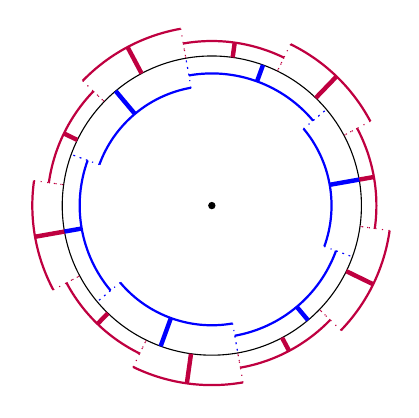
\begin{tikzpicture}[scale=1.9]
      \node (zero) at (0,0) {};
      \draw (zero) circle (1cm);

      %%%%%%%%%%%%%%%%%%%%%%%%%%%%%%%%%%%%%%%%%%%%%%%%%%%%%%%%%%%%%%%%%%%%%%%%%%%
      %%%%  Purple
      \foreach \w in {10}
      % {\foreach \sep in {0,45,90,135,180,225,270,315}
      {\foreach \sep in {0,36,72,108,144,180,216,252,288,324}
       {%\draw[thick,purple] (0,0) -- +({cos( \w + \sep )},{sin( \w + \sep )});

        \pgfmathsetmacro\r{{1.1 + mod(\w,10)/100 + mod(\sep,72)/360}}
        \draw[ultra thick,purple] ({cos( \w + \sep )},{sin( \w + \sep )})
          -- ({cos( \w + \sep) * \r},{sin( \w + \sep) * \r});

        \draw[thick,purple] ({cos( \w + \sep -18) * \r},{sin( \w + \sep -18) * \r})
          arc ({\w + \sep - 18}:{\w + \sep +18}:\r);

        \draw[dotted,purple] ({cos( \w + \sep -18) * \r},{sin( \w + \sep -18) * \r})
          -- ({cos( \w + \sep -18) * 1},{sin( \w + \sep -18) * 1});
        \draw[dotted,purple] ({cos( \w + \sep +18) * \r},{sin( \w + \sep +18) * \r})
          -- ({cos( \w + \sep +18) * 1},{sin( \w + \sep +18) * 1});
        }};

      %%%%%%%%%%%%%%%%%%%%%%%%%%%%%%%%%%%%%%%%%%%%%%%%%%%%%%%%%%%%%%%%%%%%%%%%%%%
      %%%%  Blue
      \foreach \w in {10}
      {\foreach \sep in {0,60,120,180,240,300}
       {%\draw[blue] (0,0) -- +({cos( \w + \sep ) * 0.9},{sin( \w + \sep ) * 0.9});
     
        \pgfmathsetmacro\r{{0.8 + mod(\w,10)/100 + mod(\sep,120)/720}}

        \draw[ultra thick,blue] ({cos( \w + \sep )},{sin( \w + \sep )})
          -- ({cos( \w + \sep) * \r},{sin( \w + \sep) * \r});
        \draw[thick,blue] ({cos( \w + \sep -30) * \r},{sin( \w + \sep -30) * \r})
          arc ({\w + \sep - 30}:{\w + \sep +30}:\r);


        \draw[dotted,blue] ({cos( \w + \sep -30) * \r},{sin( \w + \sep -30) * \r})
          -- ({cos( \w + \sep -30) * 1},{sin( \w + \sep -30) * 1});
        \draw[dotted,blue] ({cos( \w + \sep +30) * \r},{sin( \w + \sep +30) * \r})
          -- ({cos( \w + \sep +30) * 1},{sin( \w + \sep +30) * 1});
      }};


      % %%%%%%%%%%%%%%%%%%%%%%%%%%%%%%%%%%%%%%%%%%%%%%%%%%%%%%%%%%%%%%%%%%%%%%%%%%%
      % %%%%  Green
      % \foreach \w in {10}
      % {\foreach \sep in {0,90,180,270}
      %  {%\draw[green!60!black] (0,0) -- +({cos( \w + \sep ) * 0.8},{sin( \w + \sep) * 0.8});
     
      %   \pgfmathsetmacro\r{{0.8 + mod(\w,10)/100 + mod(\sep,180)/900}}

      %   \draw[ultra thick,green!60!black] ({cos( \w + \sep )},{sin( \w + \sep )})
      %     -- ({cos( \w + \sep) * \r},{sin( \w + \sep) * \r});
      %   \draw[thick,green!60!black] ({cos( \w + \sep -45) * \r},{sin( \w + \sep -45) * \r})
      %     arc ({\w + \sep - 45}:{\w + \sep +45}:\r);


      %   \draw[dotted,green!60!black] ({cos( \w + \sep -45) * \r},{sin( \w + \sep -45) * \r})
      %     -- ({cos( \w + \sep -45) * 1},{sin( \w + \sep -45) * 1});
      %   \draw[dotted,green!60!black] ({cos( \w + \sep +45) * \r},{sin( \w + \sep +45) * \r})
      %     -- ({cos( \w + \sep +45) * 1},{sin( \w + \sep +45) * 1});
     
      % }};

      \fill[white] (zero) circle (1.5pt);
      \fill (zero) circle (.7pt);
    \end{tikzpicture}
    \caption{$\cK=\{\textcolor{purple}{5},\textcolor{blue}{3}\}$}
  \end{subfigure}%
  \begin{subfigure}[b]{0.33\textwidth}
    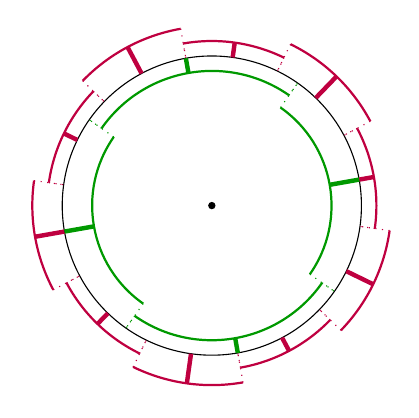
\begin{tikzpicture}[scale=1.9]
      \node (zero) at (0,0) {};
      \draw (zero) circle (1cm);

      %%%%%%%%%%%%%%%%%%%%%%%%%%%%%%%%%%%%%%%%%%%%%%%%%%%%%%%%%%%%%%%%%%%%%%%%%%%
      %%%%  Purple
      \foreach \w in {10}
      % {\foreach \sep in {0,45,90,135,180,225,270,315}
      {\foreach \sep in {0,36,72,108,144,180,216,252,288,324}
       {%\draw[thick,purple] (0,0) -- +({cos( \w + \sep )},{sin( \w + \sep )});

        \pgfmathsetmacro\r{{1.1 + mod(\w,10)/100 + mod(\sep,72)/360}}
        \draw[ultra thick,purple] ({cos( \w + \sep )},{sin( \w + \sep )})
          -- ({cos( \w + \sep) * \r},{sin( \w + \sep) * \r});

        \draw[thick,purple] ({cos( \w + \sep -18) * \r},{sin( \w + \sep -18) * \r})
          arc ({\w + \sep - 18}:{\w + \sep +18}:\r);

        \draw[dotted,purple] ({cos( \w + \sep -18) * \r},{sin( \w + \sep -18) * \r})
          -- ({cos( \w + \sep -18) * 1},{sin( \w + \sep -18) * 1});
        \draw[dotted,purple] ({cos( \w + \sep +18) * \r},{sin( \w + \sep +18) * \r})
          -- ({cos( \w + \sep +18) * 1},{sin( \w + \sep +18) * 1});
        }};

      % %%%%%%%%%%%%%%%%%%%%%%%%%%%%%%%%%%%%%%%%%%%%%%%%%%%%%%%%%%%%%%%%%%%%%%%%%%%
      % %%%%  Blue
      % \foreach \w in {10}
      % {\foreach \sep in {0,60,120,180,240,300}
      %  {%\draw[blue] (0,0) -- +({cos( \w + \sep ) * 0.9},{sin( \w + \sep ) * 0.9});
     
      %   \pgfmathsetmacro\r{{0.8 + mod(\w,10)/100 + mod(\sep,120)/720}}

      %   \draw[ultra thick,blue] ({cos( \w + \sep )},{sin( \w + \sep )})
      %     -- ({cos( \w + \sep) * \r},{sin( \w + \sep) * \r});
      %   \draw[thick,blue] ({cos( \w + \sep -30) * \r},{sin( \w + \sep -30) * \r})
      %     arc ({\w + \sep - 30}:{\w + \sep +30}:\r);


      %   \draw[dotted,blue] ({cos( \w + \sep -30) * \r},{sin( \w + \sep -30) * \r})
      %     -- ({cos( \w + \sep -30) * 1},{sin( \w + \sep -30) * 1});
      %   \draw[dotted,blue] ({cos( \w + \sep +30) * \r},{sin( \w + \sep +30) * \r})
      %     -- ({cos( \w + \sep +30) * 1},{sin( \w + \sep +30) * 1});
      % }};


      %%%%%%%%%%%%%%%%%%%%%%%%%%%%%%%%%%%%%%%%%%%%%%%%%%%%%%%%%%%%%%%%%%%%%%%%%%%
      %%%%  Green
      \foreach \w in {10}
      {\foreach \sep in {0,90,180,270}
       {%\draw[green!60!black] (0,0) -- +({cos( \w + \sep ) * 0.8},{sin( \w + \sep) * 0.8});
     
        \pgfmathsetmacro\r{{0.8 + mod(\w,10)/100 + mod(\sep,180)/900}}

        \draw[ultra thick,green!60!black] ({cos( \w + \sep )},{sin( \w + \sep )})
          -- ({cos( \w + \sep) * \r},{sin( \w + \sep) * \r});
        \draw[thick,green!60!black] ({cos( \w + \sep -45) * \r},{sin( \w + \sep -45) * \r})
          arc ({\w + \sep - 45}:{\w + \sep +45}:\r);


        \draw[dotted,green!60!black] ({cos( \w + \sep -45) * \r},{sin( \w + \sep -45) * \r})
          -- ({cos( \w + \sep -45) * 1},{sin( \w + \sep -45) * 1});
        \draw[dotted,green!60!black] ({cos( \w + \sep +45) * \r},{sin( \w + \sep +45) * \r})
          -- ({cos( \w + \sep +45) * 1},{sin( \w + \sep +45) * 1});
     
      }};

      \fill[white] (zero) circle (1.5pt);
      \fill (zero) circle (.7pt);
    \end{tikzpicture}
    \caption{$\cK=\{\textcolor{purple}{5},\textcolor{green!60!black}{2}\}$}
  \end{subfigure}%
  \begin{subfigure}[b]{0.33\textwidth}
    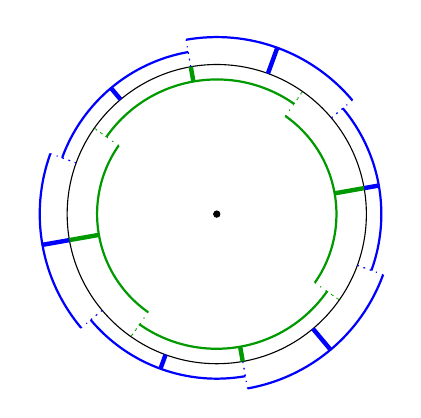
\begin{tikzpicture}[scale=1.9]
      \node (zero) at (0,0) {};
      \draw (zero) circle (1cm);

      %%%%%%%%%%%%%%%%%%%%%%%%%%%%%%%%%%%%%%%%%%%%%%%%%%%%%%%%%%%%%%%%%%%%%%%%%%%
      %%%%  Purple
      % \foreach \w in {10}
      % % {\foreach \sep in {0,45,90,135,180,225,270,315}
      % {\foreach \sep in {0,36,72,108,144,180,216,252,288,324}
      %  {%\draw[thick,purple] (0,0) -- +({cos( \w + \sep )},{sin( \w + \sep )});

      %   \pgfmathsetmacro\r{{1.1 + mod(\w,10)/100 + mod(\sep,72)/360}}
      %   \draw[ultra thick,purple] ({cos( \w + \sep )},{sin( \w + \sep )})
      %     -- ({cos( \w + \sep) * \r},{sin( \w + \sep) * \r});

      %   \draw[thick,purple] ({cos( \w + \sep -18) * \r},{sin( \w + \sep -18) * \r})
      %     arc ({\w + \sep - 18}:{\w + \sep +18}:\r);

      %   \draw[dotted,purple] ({cos( \w + \sep -18) * \r},{sin( \w + \sep -18) * \r})
      %     -- ({cos( \w + \sep -18) * 1},{sin( \w + \sep -18) * 1});
      %   \draw[dotted,purple] ({cos( \w + \sep +18) * \r},{sin( \w + \sep +18) * \r})
      %     -- ({cos( \w + \sep +18) * 1},{sin( \w + \sep +18) * 1});
      %   }};

      %%%%%%%%%%%%%%%%%%%%%%%%%%%%%%%%%%%%%%%%%%%%%%%%%%%%%%%%%%%%%%%%%%%%%%%%%%%
      %%%%  Blue
      \foreach \w in {10}
      {\foreach \sep in {0,60,120,180,240,300}
       {%\draw[blue] (0,0) -- +({cos( \w + \sep ) * 0.9},{sin( \w + \sep ) * 0.9});
     
        \pgfmathsetmacro\r{{1.1 + mod(\w,10)/100 + mod(\sep,120)/720}}

        \draw[ultra thick,blue] ({cos( \w + \sep )},{sin( \w + \sep )})
          -- ({cos( \w + \sep) * \r},{sin( \w + \sep) * \r});
        \draw[thick,blue] ({cos( \w + \sep -30) * \r},{sin( \w + \sep -30) * \r})
          arc ({\w + \sep - 30}:{\w + \sep +30}:\r);


        \draw[dotted,blue] ({cos( \w + \sep -30) * \r},{sin( \w + \sep -30) * \r})
          -- ({cos( \w + \sep -30) * 1},{sin( \w + \sep -30) * 1});
        \draw[dotted,blue] ({cos( \w + \sep +30) * \r},{sin( \w + \sep +30) * \r})
          -- ({cos( \w + \sep +30) * 1},{sin( \w + \sep +30) * 1});
      }};


      %%%%%%%%%%%%%%%%%%%%%%%%%%%%%%%%%%%%%%%%%%%%%%%%%%%%%%%%%%%%%%%%%%%%%%%%%%%
      %%%%  Green
      \foreach \w in {10}
      {\foreach \sep in {0,90,180,270}
       {%\draw[green!60!black] (0,0) -- +({cos( \w + \sep ) * 0.8},{sin( \w + \sep) * 0.8});
     
        \pgfmathsetmacro\r{{0.8 + mod(\w,10)/100 + mod(\sep,180)/900}}

        \draw[ultra thick,green!60!black] ({cos( \w + \sep )},{sin( \w + \sep )})
          -- ({cos( \w + \sep) * \r},{sin( \w + \sep) * \r});
        \draw[thick,green!60!black] ({cos( \w + \sep -45) * \r},{sin( \w + \sep -45) * \r})
          arc ({\w + \sep - 45}:{\w + \sep +45}:\r);


        \draw[dotted,green!60!black] ({cos( \w + \sep -45) * \r},{sin( \w + \sep -45) * \r})
          -- ({cos( \w + \sep -45) * 1},{sin( \w + \sep -45) * 1});
        \draw[dotted,green!60!black] ({cos( \w + \sep +45) * \r},{sin( \w + \sep +45) * \r})
          -- ({cos( \w + \sep +45) * 1},{sin( \w + \sep +45) * 1});
     
      }};

      \fill[white] (zero) circle (1.5pt);
      \fill (zero) circle (.7pt);
    \end{tikzpicture}
    \caption{$\cK=\{\textcolor{blue}{3},\textcolor{green!60!black}{2}\}$}
  \end{subfigure}
  \caption{Ideas for examples with two levels.}
\end{figure} %}}}


